% -------------------------------------------------------------------------------------------------
%      MDSG Latex Framework
%      ============================================================================================
%      File:                  introduction-[UTF8,ISO8859-1].tex
%      Author(s):             Michael Duerr
%      Version:               1
%      Creation Date:         30. Mai 2010
%      Creation Date:         30. Mai 2010
%
%      Notes:                 - Example chapter
% -------------------------------------------------------------------------------------------------
%
\chapter{Related Work}\label{sec:RelatedWork}
- Definition of field of research \\
- Scientific Scope \\
- Which comparable work in research exists? \\
- Separation from other works

\section{Reinforcement Learning}
%https://lilianweng.github.io/lil-log/2018/02/19/a-long-peek-into-reinforcement-learning.html#key-concepts
\marginpar{rl components}
Sutton and Barto wrote in ``Reinforcement learning: An introduction''\cite{suba18}
that Reinforcement learning (RL)
is based on two components that interact with each other: an environment and
an agent, see Figure \ref{fig:rl_cycle}. Those interactions take part during a
time period with discrete timesteps $t\in\mathbb{N}_0$ until a
goal is reached or the ending condition applies. Initially
the agent gets a starting environment state $S_0$, and can processes it to choose
and execute an action $A_0$. This concludes the first timestep. The environment
changes based on the action and transitions into the next state $S_{1}$. In return the the agent
receives the new state with a reward $R_{1}$ rating the action $A_0$. Afterwards the agent
proceeds to execute actions which leads to the displayed cycle of Figure \ref{fig:rl_cycle}.
\begin{figure}[hpbt]
    \centering
    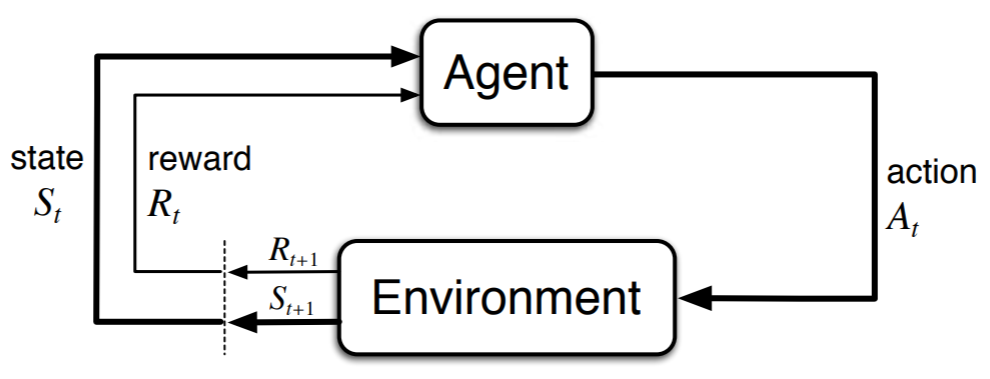
\includegraphics[width=0.6\textwidth]{pictures/RLInteractionSB}\\
    \caption[reinforcement learning cycle]{The cycle of agent-environment interaction as
        shown in ``Reinforcement learning: An introduction''\cite{suba18}}\label{fig:rl_cycle}
\end{figure}

\marginpar{sets and values}
The state $S_t$ is part of a set $S$ containing all possible environment states.
Since its likely that not all actions are valid in each environment state
the agents action selection is based on a restricted set $A_t\in A(S_t)$.
The reward $R_t$ is element of a set of possible rewards $R$, which is a subset of real
numbers $R \subset \mathbb{R}$. Therefore the reward can potentially be negative or very
low to emphasize a bad action. The general concept of RL, as defined by Sutton and
Barto, is to maximize rewards. However, unlike machine learning approaches
the agent starts with no knowledge about good or bad actions and enhances the
decision-making by aiming to improve the reward.

\marginpar{policy}
Sutton and Barto continue by defining the agents action selection with
respect to the current state as a policy $\pi$.
They explain further that a policy could be as simple as a lookup table, mapping
states to actions or it could contain a complicated search process for the best
decision. In most cases it is of stochastic nature, mapping actions and states with
probabilities. During environment interactions agents gain rewards, which then can be
used to update the policy accordingly. For example, should the reward
be low or negative it could be interpreted as a penalty. In return the policy $\pi(a \mid s)$
could then be adapted to set a very low probability for that action in combination with
that certain state. So next time the agent finds itself in that state the bad action is
not very likely to be chosen again.

\marginpar{value function}
While rewards only rate the immediate situation, a value function, i.e. the state-value
function for a policy $v_{\pi}(s)$ can be
used to estimate the long term value of a state $s$. The result is the total accumulated
reward an agent could get down the line following that state and choosing actions
based on the policy $\pi$. States that offer immediate high reward could end in
% The value function is of importance, due to states bringing high rewards could end in
low reward streaks. Or the opposite could be the case, where a low reward state
could subsequently yield high rewards. Therefore, value functions are of great use
to achieve the maximum reward.
% Other value functions can also take the executed
% action into account to reach the state from which the rewards are estimated.

\marginpar{exploration vs exploitation}
The last part to note about RL is that it entails the problem of balancing
exploration and exploitation. In order to learn, an agent has to explore the options
given. Since maximizing rewards is the goal, so an agent could become greedy
and always choose actions of which is known to result in small but positive reward.
If an agent doesn't explore enough the best action sequence will stay hidden and
if an agent always explores without exploiting the gained knowledge chances are that the
reward will not be optimal.

\section{Credit Assignment Problem}
\marginpar{intro multi problems}
Realistic RL scenarios often involve multiple agents solving problems together, for
example robots working in warehouses and factories. Such multi-agent environments come
with many difficulties. On the one hand
in a scenario where agents work independently it is very probable that they get in
each other's way in order to score highest or finish a task, preventing the overall
goal to be achieved.


In cooperative environments on the other hand, agents share the reward and therefore
can not tell who contributed useful actions and who did not. Hence all agents receive
the same reward regardless of their contribution which aggravates learning.
The independence problem is discussed in chapter \ref{market}
whereas the cooperation challenge is the focus point of this chapter.

\marginpar{coop and problem}
Sutton and Barto \cite{suba18} define a RL environment as cooperative, when agents
execute their actions collectively each timestep but receive an overall reward. In
this case individual learning is difficult or even impossible. Collective actions may
contain bad choices that could be rewarded or, in case of a penalty, good actions
that would be punished. Deciding which agent deserves more or less reward, when
splitting it up is referred to as the credit assignment problem (CAP) \cite{mi61}.

\marginpar{CAP diff kinds}
However the CAP originated in a one-agent environment that only rewarded the agent once
the goal was reached or the terminating condition applied. A popular example of this is
a chess game. In 1961, Minsky \cite{mi61} elaborated on this by explaining that a
player wins or loses the game, but cannot retrace which decision got him there.

\section{Markets}\label{market}
\marginpar{markets and advantage}
\marginpar{sm}
\marginpar{am}
\marginpar{what is expected?}